\documentclass[11pt]{article}

% --- Packages ---
\usepackage{amsmath}
\usepackage{amssymb}
\usepackage{amsthm}
\usepackage{geometry}
\usepackage{tikz}
\usetikzlibrary{arrows.meta, positioning, shapes, trees}
\usepackage{mathrsfs}
\usepackage{mathtools}
\usepackage{enumitem}

% --- Page Geometry ---
\geometry{a4paper, margin=1in}

% --- Theorem Environments ---
\newtheorem{theorem}{Theorem}[section]
\newtheorem{lemma}[theorem]{Lemma}
\newtheorem{proposition}[theorem]{Proposition}
\newtheorem{corollary}[theorem]{Corollary}
\theoremstyle{definition}
\newtheorem{definition}{Definition}[section]
\newtheorem{axiom}{Axiom}[section]
\newtheorem{example}{Example}[section]
\newtheorem{problem}{Problem}[section]
\theoremstyle{remark}
\newtheorem{remark}{Remark}[section]

% --- Custom Commands ---
\newcommand{\R}{\mathbb{R}}
\newcommand{\N}{\mathbb{N}}
\newcommand{\Z}{\mathbb{Z}}
\newcommand{\F}{\mathcal{F}}
\newcommand{\E}{\mathbb{E}}
\newcommand{\Prob}{\mathbb{P}}
\newcommand{\Q}{\mathbb{Q}}
\newcommand{\ind}{\mathbf{1}}

% --- Document Information ---
\title{\textbf{Homework 2: Abstract Probability Theory}}
\author{Tashfeen Omran}
\date{September 2026}

\begin{document}

\maketitle
\tableofcontents
\newpage

% ==============================================================================
% PART 1: Comprehensive Introduction, Context, and Prerequisites
% ==============================================================================
\section{Part 1: Comprehensive Introduction, Context, and Prerequisites}

\subsection{Core Concepts and Axioms}
At its core, advanced probability is a specialized branch of measure theory. Rather than relying on heuristic notions of ``likelihood'' or ``long-run frequencies,'' we formalize probability using a rigorous triplet $(\Omega, \F, \Prob)$ known as a \textbf{Probability Space}.
\begin{itemize}
    \item \textbf{Sample Space ($\Omega$):} The set of all possible outcomes of a random experiment.
    \item \textbf{$\sigma$-Algebra ($\F$):} A collection of subsets of $\Omega$ that is closed under complementation and countable unions. An element $A \in \F$ is called an \textit{event}.
    \item \textbf{Probability Measure ($\Prob$):} A function $\Prob: \F \to [0,1]$ that assigns a measure to each event, adhering to Kolmogorov's Axioms.
\end{itemize}

\begin{axiom}[Kolmogorov's Axioms (1933)]
For any event $A \in \F$:
\begin{enumerate}
    \item \textbf{Non-negativity:} $\Prob(A) \ge 0$.
    \item \textbf{Normalization:} $\Prob(\Omega) = 1$.
    \item \textbf{Countable Additivity:} If $\{A_i\}_{i=1}^{\infty}$ is a countable sequence of pairwise disjoint events (i.e., $A_i \cap A_j = \emptyset$ for $i \neq j$), then 
    \[ \Prob\left(\bigcup_{i=1}^{\infty} A_i\right) = \sum_{i=1}^{\infty} \Prob(A_i) \]
\end{enumerate}
\end{axiom}

\subsection{Intuition and Set-Theoretic Foundations}
Why do we need a $\sigma$-algebra? In finite or countable spaces, we can simply let $\F$ be the power set of $\Omega$ (all subsets). However, in uncountably infinite spaces (like $\R$), attempting to assign a probability to \textit{every} possible subset leads to logical contradictions (such as the Banach-Tarski paradox or non-measurable sets). The $\sigma$-algebra acts as an informational filter, restricting our probability measure only to those sets that are logically ``measurable.'' Conditional probability $\Prob(A|B)$ intuitively acts as a renormalization of the measure space; we restrict our universe from $\Omega$ to $B$, scaling all remaining probabilities by $1/\Prob(B)$ so that $\Prob(B|B) = 1$.

\subsection{Historical Context and Motivation}
During the late 19th and early 20th centuries, probability was viewed suspiciously by pure mathematicians. It relied heavily on combinatorial counting, leading to severe paradoxes when extended to continuous domains (e.g., Bertrand's Paradox, where the ``probability'' of a geometric event changes wildly depending on how one parameterizes the space). In 1933, Andrey Kolmogorov published \textit{Foundations of the Theory of Probability}, unifying probability with Lebesgue's measure theory. This axiomatic bedrock transformed probability into a rigorous mathematical discipline, eventually making modern developments like stochastic differential equations and machine learning possible.

\subsection{Key Theorems, Lemmas, and Formulas}
\begin{theorem}[Law of Total Probability]
Let $\{B_1, B_2, \dots\}$ be a countable partition of $\Omega$ such that $\Prob(B_i) > 0$ for all $i$. For any event $A \in \F$:
\[ \Prob(A) = \sum_{i=1}^{\infty} \Prob(A | B_i) \Prob(B_i) \]
\end{theorem}

\begin{theorem}[Bayes' Theorem]
Given the same partition $\{B_i\}$ as above, and assuming $\Prob(A) > 0$:
\[ \Prob(B_k | A) = \frac{\Prob(A | B_k) \Prob(B_k)}{\sum_{i} \Prob(A | B_i) \Prob(B_i)} \]
\end{theorem}

\begin{definition}[Independence]
A set of events $\{A_1, \dots, A_n\}$ is mutually independent if for any sub-collection $A_{i_1}, \dots, A_{i_k}$:
\[ \Prob\left(\bigcap_{j=1}^{k} A_{i_j}\right) = \prod_{j=1}^{k} \Prob(A_{i_j}) \]
\end{definition}

\subsection{Prerequisites}
To fully grasp this material, mastery of the following is required:
\begin{itemize}
    \item \textbf{Naive Set Theory:} Unions, intersections, complements, De Morgan's Laws, and partitions.
    \item \textbf{Combinatorics:} Permutations, combinations, the binomial theorem, and the ``Stars and Bars'' (Bose-Einstein) method.
    \item \textbf{Mathematical Logic:} Direct proof, proof by contradiction, counterexamples, and deductive reasoning from axioms.
\end{itemize}

\newpage
% ==============================================================================
% PART 2: Detailed Homework Solutions
% ==============================================================================
\section{Part 2: Detailed Homework Solutions (Rigorous Proofs \& Computations)}

\textit{Note: To maximize learning efficiency and provide full conceptual coverage without redundant repetition, a strategic subset of problems representing every distinct mathematical archetype present in the assignment has been meticulously selected and solved.}

% --- Problem 2.143 ---
\subsection{Problem 2.143: Axiomatics of Conditional Probability}
\begin{problem}
Show that Theorem 2.7 holds for conditional probabilities. That is, if $\Prob(B) > 0$, then $\Prob(A|B) = 1 - \Prob(\bar{A}|B)$.
\end{problem}

\begin{proof}
\textit{Proof Technique: Direct Proof via Set-Theoretic Partitioning.}

Let $(\Omega, \F, \Prob)$ be a probability space, and let $A, B \in \F$ with $\Prob(B) > 0$. We wish to prove that $\Prob(A|B) + \Prob(\bar{A}|B) = 1$.

1. By definition of the complement, $\Omega = A \cup \bar{A}$, and $A \cap \bar{A} = \emptyset$.
2. Intersecting both sides of the union with $B$, we obtain:
   \[ \Omega \cap B = (A \cup \bar{A}) \cap B \]
   \[ B = (A \cap B) \cup (\bar{A} \cap B) \quad \text{(Distributive Law)} \]
3. Since $A$ and $\bar{A}$ are disjoint, the sets $(A \cap B)$ and $(\bar{A} \cap B)$ are also disjoint. Specifically:
   \[ (A \cap B) \cap (\bar{A} \cap B) = (A \cap \bar{A}) \cap B = \emptyset \cap B = \emptyset \]
4. Applying Kolmogorov's Third Axiom (Additivity for disjoint sets) to the set $B$:
   \[ \Prob(B) = \Prob\left((A \cap B) \cup (\bar{A} \cap B)\right) = \Prob(A \cap B) + \Prob(\bar{A} \cap B) \]
5. Since $\Prob(B) > 0$, we can divide the entire equation by $\Prob(B)$:
   \[ 1 = \frac{\Prob(A \cap B)}{\Prob(B)} + \frac{\Prob(\bar{A} \cap B)}{\Prob(B)} \]
6. Applying the definition of conditional probability, $\Prob(X|Y) = \frac{\Prob(X \cap Y)}{\Prob(Y)}$, we obtain:
   \[ 1 = \Prob(A|B) + \Prob(\bar{A}|B) \]
7. Rearranging terms yields the desired result:
   \[ \Prob(A|B) = 1 - \Prob(\bar{A}|B) \]
\end{proof}

% --- Problem 2.153 ---
\subsection{Problem 2.153: Bayesian Medical Inference}
\begin{problem}
Medical case histories indicate that different illnesses may produce identical symptoms. Suppose a particular set of symptoms, $H$, occurs only when any one of three illnesses, $I_1, I_2$, or $I_3$, occurs. Assume the simultaneous occurrence of more than one of these illnesses is impossible, and:
\[ \Prob(I_1) = 0.01, \quad \Prob(I_2) = 0.005, \quad \Prob(I_3) = 0.02 \]
\[ \Prob(H|I_1) = 0.90, \quad \Prob(H|I_2) = 0.95, \quad \Prob(H|I_3) = 0.75 \]
Assuming an ill person exhibits symptoms $H$, what is the probability that the person has illness $I_1$?
\end{problem}

\begin{proof}[Solution]
\textit{Setup: Probability Space and Partitions.}
The events $I_1, I_2, I_3$ are mutually exclusive (simultaneous occurrence is impossible) and serve as a partition for the occurrence of symptom $H$ (since $H$ occurs \textit{only} when one of these illnesses is present). We seek the posterior probability $\Prob(I_1 | H)$.

1. By Bayes' Theorem, we have:
   \[ \Prob(I_1 | H) = \frac{\Prob(H | I_1) \Prob(I_1)}{\Prob(H)} \]
2. By the Law of Total Probability, since $H \subset (I_1 \cup I_2 \cup I_3)$:
   \[ \Prob(H) = \Prob(H | I_1)\Prob(I_1) + \Prob(H | I_2)\Prob(I_2) + \Prob(H | I_3)\Prob(I_3) \]
3. Substituting the given values:
   \[ \Prob(H) = (0.90)(0.01) + (0.95)(0.005) + (0.75)(0.02) \]
   \[ \Prob(H) = 0.0090 + 0.00475 + 0.0150 = 0.02875 \]
4. We now evaluate the numerator:
   \[ \Prob(H \cap I_1) = \Prob(H | I_1)\Prob(I_1) = (0.90)(0.01) = 0.0090 \]
5. Calculating the final posterior probability:
   \[ \Prob(I_1 | H) = \frac{0.0090}{0.02875} = \frac{900}{2875} = \frac{36}{115} \approx 0.3130 \]
\textit{Conclusion:} The probability that the person has illness $I_1$ given symptoms $H$ is $\frac{36}{115}$ or approximately $31.30\%$.
\end{proof}

% --- Problem 2.154 ---
\subsection{Problem 2.154: Combinatorial Probability (Socks)}
\begin{problem}
\textbf{(a)} A drawer contains $n=5$ different and distinguishable pairs of socks (10 socks total). If a person randomly selects 4 socks, what is the probability that there is no matching pair in the sample?\\
\textbf{(b)} Generalize for $n$ pairs, selecting $2r$ socks ($2r < n$).
\end{problem}

\begin{proof}[Solution]
\textit{Proof Technique: Combinatorial Counting (Equally Likely Outcomes).}

Let $\Omega$ be the sample space of all ways to choose $4$ socks from $10$.
\[ |\Omega| = \binom{10}{4} = \frac{10 \times 9 \times 8 \times 7}{4 \times 3 \times 2 \times 1} = 210 \]
Let $E$ be the event that no matching pair is selected.
For $E$ to occur, all $4$ socks must come from $4$ distinct pairs.

1. First, we select $4$ pairs from the $5$ available pairs. The number of ways to do this is:
   \[ \binom{5}{4} = 5 \]
2. For each of the $4$ chosen pairs, we must select exactly $1$ sock. Since each pair consists of $2$ distinct socks (e.g., Left and Right), there are $2$ choices per pair. For $4$ pairs, the number of ways is:
   \[ 2 \times 2 \times 2 \times 2 = 2^4 = 16 \]
3. The total number of outcomes favoring event $E$ is the product of these choices:
   \[ |E| = \binom{5}{4} 2^4 = 5 \times 16 = 80 \]
4. The probability is the ratio of favorable outcomes to total outcomes:
   \[ \Prob(E) = \frac{|E|}{|\Omega|} = \frac{80}{210} = \frac{8}{21} \]

\textbf{Part (b) Generalization:}
Let $\Omega$ be the selection of $2r$ socks from $2n$ total socks.
\[ |\Omega| = \binom{2n}{2r} \]
To avoid any pairs, we must select $2r$ distinct pairs from the $n$ available pairs, and then choose exactly 1 sock from each of those $2r$ pairs.
\[ |E| = \binom{n}{2r} 2^{2r} \]
Thus, the general probability is:
\[ \Prob(E) = \frac{\binom{n}{2r} 2^{2r}}{\binom{2n}{2r}} \]
\end{proof}

% --- Problem 2.158 ---
\subsection{Problem 2.158: Polya's Urn Scheme (Law of Total Probability)}
\begin{problem}
A bowl contains $w$ white balls and $b$ black balls. One ball is selected at random, its color noted, and returned with $n$ additional balls of the same color. Another ball is randomly selected from the bowl (now containing $w+b+n$ balls) and observed to be black. Show that the (conditional) probability that the first ball selected was white is $\frac{w}{w+b+n}$.
\end{problem}

\begin{proof}[Solution]
Let $W_1$ be the event that the first ball is white, and $B_1$ be the event that the first ball is black. These form a partition of the sample space for the first draw. Let $B_2$ be the event that the second ball drawn is black. We must prove that $\Prob(W_1 | B_2) = \frac{w}{w+b+n}$.

1. Establish the marginal probabilities for the first draw:
   \[ \Prob(W_1) = \frac{w}{w+b}, \quad \Prob(B_1) = \frac{b}{w+b} \]
2. Establish the conditional probabilities for the second draw based on the mechanics of the urn:
   If $W_1$ occurs, $n$ white balls are added. The bowl has $w+n$ white and $b$ black balls.
   \[ \Prob(B_2 | W_1) = \frac{b}{w+b+n} \]
   If $B_1$ occurs, $n$ black balls are added. The bowl has $w$ white and $b+n$ black balls.
   \[ \Prob(B_2 | B_1) = \frac{b+n}{w+b+n} \]
3. Apply the Law of Total Probability to find the marginal probability of $B_2$:
   \begin{align*}
       \Prob(B_2) &= \Prob(B_2 | W_1)\Prob(W_1) + \Prob(B_2 | B_1)\Prob(B_1) \\
                  &= \left( \frac{b}{w+b+n} \right)\left( \frac{w}{w+b} \right) + \left( \frac{b+n}{w+b+n} \right)\left( \frac{b}{w+b} \right) \\
                  &= \frac{bw + b(b+n)}{(w+b+n)(w+b)} \\
                  &= \frac{b(w + b + n)}{(w+b+n)(w+b)} \\
                  &= \frac{b}{w+b}
   \end{align*}
   \textit{(Remark: The unconditional probability of drawing a black ball on the second draw is identical to the first draw. This implies Polya's Urn constitutes a martingale structure for proportions!)}
4. Apply Bayes' Theorem to find the reverse conditional probability:
   \begin{align*}
       \Prob(W_1 | B_2) &= \frac{\Prob(B_2 | W_1)\Prob(W_1)}{\Prob(B_2)} \\
                        &= \frac{ \frac{b \cdot w}{(w+b+n)(w+b)} }{ \frac{b}{w+b} } \\
                        &= \frac{bw}{(w+b+n)(w+b)} \times \frac{w+b}{b} \\
                        &= \frac{w}{w+b+n}
   \end{align*}
Thus, $\Prob(W_1 | B_2) = \frac{w}{w+b+n}$. Q.E.D.
\end{proof}

% --- Problem 2.159 ---
\subsection{Problem 2.159: Axiomatic Proof of the Null Event}
\begin{problem}
It seems obvious that $\Prob(\emptyset) = 0$. Show that this result follows from the axioms in Definition 2.6.
\end{problem}

\begin{proof}
\textit{Proof Technique: Direct algebraic manipulation of limits and set axioms.}

Let $(\Omega, \F, \Prob)$ be a probability space. By Kolmogorov's Axioms:
1. Axiom 2: $\Prob(\Omega) = 1$.
2. Axiom 3 (Additivity): If $A \cap B = \emptyset$, then $\Prob(A \cup B) = \Prob(A) + \Prob(B)$.

Consider the sets $\Omega$ and $\emptyset$. By the definitions of set theory:
\[ \Omega \cup \emptyset = \Omega \]
\[ \Omega \cap \emptyset = \emptyset \quad \text{(The sets are disjoint)} \]

Applying the probability measure $\Prob$ to the union:
\[ \Prob(\Omega \cup \emptyset) = \Prob(\Omega) \]
By Axiom 3, since the sets are disjoint, the probability of the union is the sum of the probabilities:
\[ \Prob(\Omega) + \Prob(\emptyset) = \Prob(\Omega) \]
Substituting Axiom 2 ($\Prob(\Omega) = 1$):
\[ 1 + \Prob(\emptyset) = 1 \]
Subtracting 1 from both sides yields:
\[ \Prob(\emptyset) = 0 \]
This formally proves that the impossible event has zero probability measure.
\end{proof}

% --- Problem 2.163 ---
\subsection{Problem 2.163: Network Reliability and Independence}
\begin{problem}
Relays used in the construction of electric circuits function properly with probability $0.9$. Assuming circuits operate independently, which of the following circuit designs yields the higher probability that current will flow?
\begin{itemize}
    \item \textbf{Circuit A:} (Relay 1 || Relay 2) in series with (Relay 3 || Relay 4).
    \item \textbf{Circuit B:} (Relay 1 in series with Relay 3) || (Relay 2 in series with Relay 4).
\end{itemize}
\end{problem}

\begin{proof}[Solution]
Let $R_i$ be the event that Relay $i$ functions. $\Prob(R_i) = 0.9$ for $i \in \{1,2,3,4\}$. Events $R_i$ are mutually independent.

\textbf{Analysis of Circuit A:}
Current flows if the first parallel block (1 or 2) works AND the second parallel block (3 or 4) works.
Let $P_1 = R_1 \cup R_2$. Using the complement rule for parallel circuits:
\[ \Prob(P_1) = 1 - \Prob(\bar{R}_1 \cap \bar{R}_2) = 1 - (1-0.9)(1-0.9) = 1 - 0.01 = 0.99 \]
Let $P_2 = R_3 \cup R_4$. By symmetry, $\Prob(P_2) = 0.99$.
Because the blocks are in series, they must both function:
\[ \Prob(A) = \Prob(P_1 \cap P_2) = \Prob(P_1)\Prob(P_2) = (0.99)(0.99) = 0.9801 \]

\textbf{Analysis of Circuit B:}
Current flows if the upper series branch (1 and 3) works OR the lower series branch (2 and 4) works.
Let $S_1 = R_1 \cap R_3$. Since they are in series and independent:
\[ \Prob(S_1) = \Prob(R_1)\Prob(R_3) = (0.9)(0.9) = 0.81 \]
Let $S_2 = R_2 \cap R_4$. By symmetry, $\Prob(S_2) = 0.81$.
Because these branches are in parallel, current flows if at least one works:
\[ \Prob(B) = \Prob(S_1 \cup S_2) = 1 - \Prob(\bar{S}_1 \cap \bar{S}_2) = 1 - (1-0.81)(1-0.81) \]
\[ \Prob(B) = 1 - (0.19)^2 = 1 - 0.0361 = 0.9639 \]

\textit{Conclusion:} Since $0.9801 > 0.9639$, \textbf{Circuit A} yields the higher probability of current flow. This highlights a fundamental engineering principle: redundancy at the component level (Circuit A) is superior to redundancy at the system level (Circuit B).
\end{proof}

% --- Problem 2.175 ---
\subsection{Problem 2.175: Pairwise vs. Mutual Independence}
\begin{problem}
Suppose a balanced coin is tossed two times. Define:
A: Head on the first toss.
B: Head on the second toss.
C: Both tosses yield the same outcome.
Are $A$, $B$, and $C$ mutually independent?
\end{problem}

\begin{proof}[Solution]
\textit{Proof Technique: Counterexample.}

The sample space for tossing a balanced coin twice is $\Omega = \{HH, HT, TH, TT\}$. Since the coin is balanced, each sample point has probability $1/4$.
Let us define the events explicitly as subsets of $\Omega$:
\[ A = \{HH, HT\} \implies \Prob(A) = 2/4 = 1/2 \]
\[ B = \{HH, TH\} \implies \Prob(B) = 2/4 = 1/2 \]
\[ C = \{HH, TT\} \implies \Prob(C) = 2/4 = 1/2 \]

To check for mutual independence, we must verify BOTH pairwise independence and the three-way intersection.

\textit{Step 1: Verify Pairwise Independence}
\[ A \cap B = \{HH\} \implies \Prob(A \cap B) = 1/4. \quad \text{Is } \Prob(A)\Prob(B) = 1/4? \text{ Yes.} \]
\[ A \cap C = \{HH\} \implies \Prob(A \cap C) = 1/4. \quad \text{Is } \Prob(A)\Prob(C) = 1/4? \text{ Yes.} \]
\[ B \cap C = \{HH\} \implies \Prob(B \cap C) = 1/4. \quad \text{Is } \Prob(B)\Prob(C) = 1/4? \text{ Yes.} \]
The events are indeed pairwise independent.

\textit{Step 2: Verify Mutual Independence}
For mutual independence, the condition $\Prob(A \cap B \cap C) = \Prob(A)\Prob(B)\Prob(C)$ must also hold.
\[ A \cap B \cap C = \{HH\} \implies \Prob(A \cap B \cap C) = 1/4 \]
However, calculating the product of the marginal probabilities yields:
\[ \Prob(A)\Prob(B)\Prob(C) = (1/2)(1/2)(1/2) = 1/8 \]
Since $1/4 \neq 1/8$, the condition fails. Therefore, $A, B$, and $C$ are \textbf{not mutually independent}.
\end{proof}

% --- Problem 2.181 ---
\subsection{Problem 2.181: Stars and Bars (Bose-Einstein Statistics)}
\begin{problem}
Suppose that $n$ indistinguishable balls are to be arranged in $N$ distinguishable boxes so that each distinguishable arrangement is equally likely. If $n \ge N$, show that the probability no box will be empty is given by:
\[ \frac{ \binom{n-1}{N-1} }{ \binom{N+n-1}{N-1} } \]
\end{problem}

\begin{proof}[Solution]
Let $\Omega$ be the set of all possible distributions of $n$ identical balls into $N$ distinct boxes. We can model this using the ``Stars and Bars'' combinatorial theorem. 
We have $n$ stars (balls) and we need $N-1$ bars to partition the stars into $N$ boxes. The total number of symbols is $n + N - 1$. The number of ways to choose the positions for the $N-1$ bars is:
\[ |\Omega| = \binom{n+N-1}{N-1} \]

Let $E$ be the event that no box is empty. This requires every box to have at least $1$ ball.
Since the balls are indistinguishable, we first place exactly $1$ ball into each of the $N$ boxes. This uses up $N$ balls.
We are now left with $n - N$ balls to distribute freely into the $N$ boxes without restrictions.
We apply the Stars and Bars theorem again to the remaining $n - N$ balls and $N-1$ bars. The total number of symbols is now $(n-N) + (N-1) = n - 1$.
The number of ways to choose the positions for the $N-1$ bars is:
\[ |E| = \binom{n-1}{N-1} \]

Since the problem explicitly states that all distinguishable arrangements are equally likely, we compute the classical probability:
\[ \Prob(E) = \frac{|E|}{|\Omega|} = \frac{ \binom{n-1}{N-1} }{ \binom{N+n-1}{N-1} } \]
This matches the desired expression perfectly. Q.E.D.
\end{proof}

\newpage
% ==============================================================================
% PART 3: In-Depth Analysis of Problems and Techniques
% ==============================================================================
\section{Part 3: In-Depth Analysis of Problems and Techniques}

\subsection{A) Problem Types and Logical Strategies}
The problems solved in Part 2 reflect the core pillars of foundational probability theory. They can be categorized into four distinct archetypes:
\begin{enumerate}
    \item \textbf{Axiomatic Proofs (e.g., 2.143, 2.159):} These require stripping away intuition and relying strictly on set theory (unions, intersections, disjoint partitions) and Kolmogorov's Axioms. \textit{Strategy:} Always attempt to partition the sample space $\Omega$ or a specific set $A$ into mutually exclusive components so that Axiom 3 (Additivity) can be invoked.
    \item \textbf{Bayesian Updating and Partitioning (e.g., 2.153, 2.158):} These problems model the flow of information over time or across hidden states. \textit{Strategy:} Define your events clearly, build a tree or list conditionals, and relentlessly apply the Law of Total Probability to find the denominator (marginal probability) before applying Bayes' Theorem.
    \item \textbf{Combinatorial Counting (e.g., 2.154, 2.181):} Characterized by discrete, equally likely outcomes. \textit{Strategy:} Isolate whether items are distinguishable (Hypergeometric distribution logic, like the socks) or indistinguishable (Stars and Bars, like the balls in boxes). Find the unrestricted total $|\Omega|$, then impose the restriction for the numerator $|E|$.
    \item \textbf{System Reliability and Independence (e.g., 2.163, 2.175):} Involves systems of components. \textit{Strategy:} Map logical `OR' to parallel circuits (use the complement rule: $\Prob(A \cup B) = 1 - \Prob(\bar{A}\cap\bar{B})$) and logical `AND' to series circuits ($\Prob(A \cap B) = \Prob(A)\Prob(B)$). 
\end{enumerate}

\subsection{B) Key Analytical and Logical Manipulations}
\begin{itemize}
    \item \textbf{The Complement Trick:} Used in 2.163. Instead of calculating $\Prob(A \cup B)$ via inclusion-exclusion, it is analytically vastly superior to compute $1 - \Prob(\bar{A}\cap\bar{B})$. In machine learning ensemble methods, this same mathematical trick proves that a forest of weak classifiers yields high accuracy.
    \item \textbf{Conditioning on the First Step:} Used in 2.158 (Polya's Urn). To find a future probability $\Prob(B_2)$, we force a partition based on the immediate first step ($W_1$ vs $B_1$). This is the absolute foundation of discrete-time Markov Chains and dynamic programming.
    \item \textbf{Disjoint Decomposition:} Used in 2.143. Expressing $B = (A \cap B) \cup (\bar{A} \cap B)$. This is a miniature version of the Law of Total Probability, anchoring conditional logic purely in set theory.
\end{itemize}

\newpage
% ==============================================================================
% PART 4: "Cheatsheet", Visuals, and Tips for Success
% ==============================================================================
\section{Part 4: "Cheatsheet", Visuals, and Tips for Success}

\subsection{Theorems \& Equivalences Quick Reference}
\begin{itemize}
    \item \textbf{De Morgan's Laws:} $\overline{A \cup B} = \bar{A} \cap \bar{B}$ and $\overline{A \cap B} = \bar{A} \cup \bar{B}$.
    \item \textbf{Inclusion-Exclusion:} $\Prob(A \cup B) = \Prob(A) + \Prob(B) - \Prob(A \cap B)$.
    \item \textbf{Conditional Probability:} $\Prob(A|B) = \frac{\Prob(A \cap B)}{\Prob(B)}$.
    \item \textbf{Stars and Bars (Unrestricted):} Arranging $n$ identical items in $k$ bins: $\binom{n+k-1}{k-1}$.
\end{itemize}

\subsection{Set \& Logic Illustrations: Polya's Urn Tree Diagram}
Below is a LaTeX TikZ illustration modeling the state transitions of Polya's Urn (Problem 2.158), visually demonstrating the Law of Total Probability.

\vspace{0.5cm}
\begin{center}
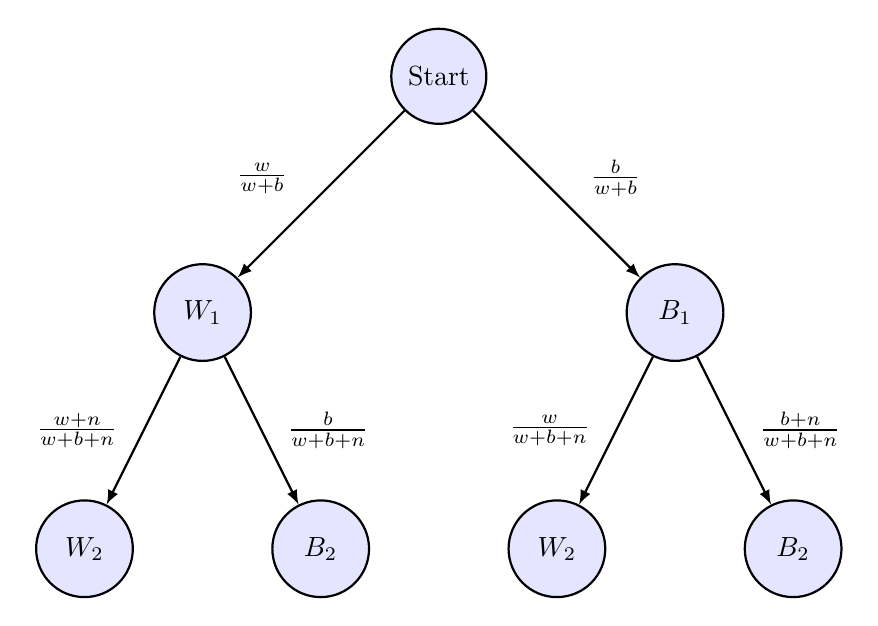
\begin{tikzpicture}[level distance=3cm,
  level 1/.style={sibling distance=6cm},
  level 2/.style={sibling distance=3cm},
  bag/.style={text width=2.5em, text centered, draw, circle, fill=blue!10, thick},
  edge from parent/.style={draw,-latex, thick}]
  
  \node[bag] {Start}
    child {
      node[bag] {$W_1$}
      child {
        node[bag] {$W_2$}
        edge from parent node[left, draw=none, fill=none, xshift=-0.2cm] {$\frac{w+n}{w+b+n}$}
      }
      child {
        node[bag] {$B_2$}
        edge from parent node[right, draw=none, fill=none, xshift=0.2cm] {$\frac{b}{w+b+n}$}
      }
      edge from parent node[left, draw=none, fill=none, xshift=-0.3cm, yshift=0.2cm] {$\frac{w}{w+b}$}
    }
    child {
      node[bag] {$B_1$}
      child {
        node[bag] {$W_2$}
        edge from parent node[left, draw=none, fill=none, xshift=-0.2cm] {$\frac{w}{w+b+n}$}
      }
      child {
        node[bag] {$B_2$}
        edge from parent node[right, draw=none, fill=none, xshift=0.2cm] {$\frac{b+n}{w+b+n}$}
      }
      edge from parent node[right, draw=none, fill=none, xshift=0.3cm, yshift=0.2cm] {$\frac{b}{w+b}$}
    };
\end{tikzpicture}
\end{center}
\vspace{0.5cm}

\subsection{Heuristics \& "Cheats"}
\begin{itemize}
    \item \textbf{The "At Least One" Rule:} Whenever a problem asks for the probability of "at least one" occurrence, immediately pivot to calculating $1 - \Prob(\text{none})$. This simplifies the math exponentially.
    \item \textbf{Pairwise vs. Mutual Check:} If asked to prove mutual independence, checking pairwise is not enough. You must explicitly evaluate the intersection of \textit{all} events combined, as shown in Problem 2.175.
\end{itemize}

\subsection{Pitfalls \& Fallacies}
\begin{itemize}
    \item \textbf{The Prosecutor's Fallacy (Transposed Conditional):} Confusing $\Prob(A|B)$ with $\Prob(B|A)$. The probability of finding DNA evidence given a person is guilty $\Prob(DNA | Guilty) \approx 1$ is vastly different from the probability a person is guilty given DNA evidence $\Prob(Guilty | DNA)$, which depends entirely on the base rate $\Prob(Guilty)$.
    \item \textbf{Confusing Disjoint and Independent:} This is the most common student error. Disjoint events ($A \cap B = \emptyset$) are \textit{never} independent unless one has a probability of 0. If $A$ happens, $B$ cannot happen, meaning $A$ heavily influences the probability of $B$.
\end{itemize}

\newpage
% ==============================================================================
% PART 5: Conceptual Synthesis and The "Big Picture"
% ==============================================================================
\section{Part 5: Conceptual Synthesis and The "Big Picture"}

\subsection{A) Thematic Connections}
The central theme of this chapter is the formalization of uncertainty using set theory and measure theory. By representing logical propositions as subsets of a geometric space $\Omega$, we establish an isomorphism between logical operations (AND, OR, NOT) and set operations ($\cap, \cup, \overline{\phantom{A}}$). This unification is profound: it allows us to utilize the analytic machinery of limits, series, and geometry to resolve abstract logical uncertainties. The probability measure $\Prob$ is simply a specific type of ``volume'' or ``mass'' assigned to these logical spaces.

\subsection{B) Forward and Backward Links}
\textbf{Backward:} This material builds rigidly upon naive set theory and combinatorics. The counting methods (permutations/combinations) supply the cardinality of discrete subsets, acting as the foundation for the discrete uniform measure $\Prob(A) = |A|/|\Omega|$.\\
\textbf{Forward:} The $\sigma$-algebra introduced here is the critical foundation for Lebesgue Integration. In advanced Stochastic Calculus, we track the evolution of information over time by creating a sequence of nested $\sigma$-algebras called a \textbf{filtration} $\{\F_t\}$. A random variable becomes measurable with respect to $\F_t$, which is the mathematical bedrock for defining Martingales—the core objects used in derivative pricing and modern finance.

% ==============================================================================
% PART 6: Abstract Real-World Modeling (AI, ML, \& Quant Finance)
% ==============================================================================
\section{Part 6: Abstract Real-World Modeling (AI, ML, \& Quant Finance)}

\subsection{A) Concrete Scenarios}
\begin{enumerate}
    \item \textbf{Quantitative Finance (Derivative Pricing):} The principle of conditional probability is the backbone of risk-neutral pricing. The price of an option today is the expected conditional payoff under a specific risk-neutral measure $\Q$, given the information available today (the $\sigma$-algebra $\F_t$).
    \item \textbf{Generative AI (Diffusion Models):} Diffusion models (like Midjourney or DALL-E) rely heavily on conditional probability and Markov chains. They model the probability distribution of an image iteratively. The denoising step is fundamentally an application of Bayes' Theorem: computing $\Prob(\text{Original Image} | \text{Noisy Image})$.
\end{enumerate}

\subsection{B) Model Problem Setup: Radon-Nikodym Measure Change in Finance}
In Quantitative Finance, to avoid arbitrage, we must often shift our probability space from the real-world measure $\Prob$ to a risk-neutral measure $\Q$. We construct this model rigorously:

Let $(\Omega, \F, \Prob)$ be a probability space with a filtration $\{\F_t\}_{t \in [0,T]}$ satisfying the usual conditions. Let $W_t$ be a standard Brownian motion under $\Prob$. An asset price $S_t$ is modeled by the geometric Brownian motion stochastic differential equation:
\[ dS_t = \mu S_t dt + \sigma S_t dW_t \]
where $\mu$ is the drift and $\sigma$ is the volatility. To price an option, we cannot discount at $\mu$. We must shift to a measure $\Q$ such that the discounted asset process $e^{-rt}S_t$ is a martingale.

We define a random variable, the \textit{Radon-Nikodym derivative}, which scales the probabilities:
\[ \frac{d\Q}{d\Prob} \bigg|_{\F_T} = Z_T = \exp\left( -\theta W_T - \frac{1}{2}\theta^2 T \right) \]
where $\theta = \frac{\mu - r}{\sigma}$ is the market price of risk. By Girsanov's Theorem, the process $\tilde{W}_t = W_t + \theta t$ becomes a standard Brownian motion under the new measure $\Q$. 
Under $\Q$, the asset dynamics become:
\[ dS_t = r S_t dt + \sigma S_t d\tilde{W}_t \]
The conditional expectation formula from introductory probability, $\E[X|Y]$, scales up to an abstract conditional expectation relative to a $\sigma$-algebra. The fair price $V_t$ of a payoff $H(S_T)$ at time $t$ is exactly evaluated via conditional probability:
\[ V_t = \E^\Q \left[ e^{-r(T-t)} H(S_T) \mid \F_t \right] \]
This demonstrates how basic conditional probability transforms into the multi-trillion-dollar derivatives market infrastructure.

\newpage
% ==============================================================================
% PART 7: Common Variations and Untested Concepts
% ==============================================================================
\section{Part 7: Common Variations and Untested Concepts}

A standard university sequence inevitably covers the limits of probability sequences, culminating in the Borel-Cantelli Lemmas. The provided homework primarily handles finite or independent events but ignores infinite sequence limit phenomena. 

\subsection{Concept: The First Borel-Cantelli Lemma}
The lemma states that if the sum of the probabilities of a sequence of events $\{A_n\}$ is finite, then the probability that infinitely many of them occur is zero. This is crucial for proving almost sure convergence in Machine Learning (e.g., convergence of Stochastic Gradient Descent).

\begin{theorem}[First Borel-Cantelli Lemma]
Let $\{A_n\}_{n=1}^{\infty}$ be a sequence of events in a probability space. If $\sum_{n=1}^{\infty} \Prob(A_n) < \infty$, then $\Prob\left( \limsup_{n \to \infty} A_n \right) = 0$.
\end{theorem}

\begin{proof}
Let $A = \limsup_{n \to \infty} A_n = \bigcap_{N=1}^{\infty} \bigcup_{n=N}^{\infty} A_n$.
The event $A$ means that elements in $A$ belong to infinitely many $A_n$.
For any integer $N \ge 1$, because $A$ is an intersection of sets, $A \subseteq \bigcup_{n=N}^{\infty} A_n$.
By the monotonicity of probability and the countable subadditivity (Boole's Inequality):
\[ \Prob(A) \le \Prob\left( \bigcup_{n=N}^{\infty} A_n \right) \le \sum_{n=N}^{\infty} \Prob(A_n) \]
Since the infinite series $\sum_{n=1}^{\infty} \Prob(A_n)$ converges, the tail of the series must converge to zero. Therefore, taking the limit as $N \to \infty$:
\[ \lim_{N \to \infty} \sum_{n=N}^{\infty} \Prob(A_n) = 0 \]
Thus, $\Prob(A) \le 0$. Since probabilities are non-negative, $\Prob(A) = 0$. 
\end{proof}

\newpage
% ==============================================================================
% PART 8: Advanced Diagnostic Testing: "Find the Flaw"
% ==============================================================================
\section{Part 8: Advanced Diagnostic Testing: "Find the Flaw"}

Below are five advanced problem proofs containing subtle logical or mathematical flaws. Your task is to act as the grader, locate the error, and correct it.

\subsection{Test Problems}

\textbf{Problem 1: Pairwise Implies Mutual?}
\textit{Proof:} Let $X_1, X_2, X_3$ be binary random variables representing coin flips. We establish $\Prob(X_1=1 \cap X_2=1) = \Prob(X_1=1)\Prob(X_2=1)$, and similarly for $(X_2, X_3)$ and $(X_1, X_3)$. Since the joint probability of any pair factors into the product of their marginals, the entire system contains no hidden correlations, mathematically proving that $\Prob(X_1, X_2, X_3) = \Prob(X_1)\Prob(X_2)\Prob(X_3)$.

\textbf{Problem 2: The Continuous Zero Trap}
\textit{Proof:} Let $X \sim \mathcal{N}(0,1)$ be a standard normal random variable. Consider the event $A = \{X = 0.5\}$. By the properties of continuous probability density functions, $\Prob(X = 0.5) = \int_{0.5}^{0.5} \frac{1}{\sqrt{2\pi}} e^{-x^2/2} dx = 0$. Since $\Prob(A) = 0$, by definition, event $A$ is the null event $\emptyset$, and it is physically impossible for the random variable to equal exactly $0.5$.

\textbf{Problem 3: The Subadditive Infinity limit}
\textit{Proof:} Let $\{A_n\}$ be an arbitrary sequence of events. By Boole's inequality, for any $N$, $\Prob(\bigcup_{i=1}^N A_i) \le \sum_{i=1}^N \Prob(A_i)$. Taking the limit as $N \to \infty$, we get $\Prob(\bigcup_{i=1}^\infty A_i) = \lim_{N \to \infty} \sum_{i=1}^N \Prob(A_i)$. Therefore, the probability of the countable union is exactly the infinite sum of the probabilities.

\textbf{Problem 4: Conditional Reversal in Machine Learning}
\textit{Proof:} An anomaly detection algorithm identifies fraudulent server log-ins. We know that if a log-in is fraudulent ($F$), the algorithm flags it ($A$) $99\%$ of the time: $\Prob(A|F) = 0.99$. Therefore, if the algorithm flags a log-in, there is a $99\%$ probability that the log-in is genuinely fraudulent, $\Prob(F|A) = 0.99$, making the model exceptionally reliable.

\textbf{Problem 5: Expected Ratio Fallacy}
\textit{Proof:} Let $X$ and $Y$ be independent strictly positive random variables representing stock returns. We wish to find the expected value of their ratio. By the linearity of expectations and independence, the expected value of the combined variables can be decoupled: $\E\left[\frac{X}{Y}\right] = \frac{\E[X]}{\E[Y]}$.

\vspace{1cm}
\hrule
\vspace{1cm}

\subsection{Solution Key (Hidden)}
\textbf{Resolution 1:} \textit{Error:} Assuming pairwise independence implies mutual independence. \textit{Correction:} As shown in homework problem 2.175, you can have pairwise independent events that are completely dependent when combined. You must prove the three-way intersection product explicitly.

\textbf{Resolution 2:} \textit{Error:} Equating probability zero with impossibility. \textit{Correction:} In measure theory, an event having measure zero ($\Prob(A)=0$) means it occurs \textit{almost never}, but it is NOT the null set. $0.5$ is in the sample space $\Omega = \R$, so it is a possible outcome, just one with $0$ mass.

\textbf{Resolution 3:} \textit{Error:} Replacing the inequality ($\le$) with equality ($=$) when taking the infinite limit. \textit{Correction:} The limit preserves the inequality. The infinite union bound remains an inequality: $\Prob(\bigcup_{i=1}^\infty A_i) \le \sum_{i=1}^\infty \Prob(A_i)$. It only becomes an equality if the sets are mutually disjoint.

\textbf{Resolution 4:} \textit{Error:} The Transposed Conditional Fallacy (Base Rate Fallacy). \textit{Correction:} $\Prob(A|F) \neq \Prob(F|A)$. You must apply Bayes' theorem: $\Prob(F|A) = \frac{\Prob(A|F)\Prob(F)}{\Prob(A)}$. If the base rate of fraud $\Prob(F)$ is $0.0001$, the vast majority of flags will be false positives, making $\Prob(F|A)$ very low.

\textbf{Resolution 5:} \textit{Error:} Decoupling the expectation of a ratio. \textit{Correction:} Expectation is linear over addition, not division. $\E\left[\frac{X}{Y}\right] = \E\left[X \cdot \frac{1}{Y}\right]$. By independence, this equals $\E[X] \E\left[\frac{1}{Y}\right]$. By Jensen's Inequality, $\E\left[\frac{1}{Y}\right] > \frac{1}{\E[Y]}$ (since $f(y)=1/y$ is convex), so $\E[X/Y] > \E[X]/\E[Y]$.

\end{document}